\documentclass{article}    
\usepackage[letterpaper,margin=1in]{geometry}
\usepackage{lastpage}
\usepackage{graphicx}
\usepackage{fancyhdr}
\usepackage{enumitem}
\usepackage{amssymb}
\usepackage{amsmath}

\def\ojoin{\setbox0=\hbox{$\bowtie$}%
  \rule[-.02ex]{.25em}{.4pt}\llap{\rule[\ht0]{.25em}{.4pt}}}
\def\leftouterjoin{\mathbin{\ojoin\mkern-5.8mu\bowtie}}
\def\rightouterjoin{\mathbin{\bowtie\mkern-5.8mu\ojoin}}
\def\fullouterjoin{\mathbin{\ojoin\mkern-5.8mu\bowtie\mkern-5.8mu\ojoin}}

\fancypagestyle{plain}{%
\fancyhf{}%
\lhead{ECS165A SQ18}
\rhead{\today}
\cfoot{Homework 4\\ \thepage\ of \pageref{LastPage} }
\renewcommand{\headrulewidth}{0.4pt}
\renewcommand{\footrulewidth}{0.4pt}
}

\pagestyle{fancy}
\fancyhf{}
\lhead{ECS165A SQ18}
\rhead{\today}
\cfoot{Homework 4\\ \thepage\ of \pageref{LastPage} }
\renewcommand{\headrulewidth}{0.4pt}
\renewcommand{\footrulewidth}{0.4pt}

\begin{document}

\title{Homework 4}
\author{Name: Miguel Salazar\\SID: 998915375\\Partner Name: Jennifer Wong\\Partner SID: 913160121}

\maketitle

Due 11:59PM June 5, 2018. {\bf READ ALL DIRECTIONS VERY CAREFULLY!} 
Submit your code, tex files along with a generated PDF. {\bf DO NOT SUBMIT DATA FILES!} 
For this homework you will be working in groups of two, a group of three will only be allowed with approval due to odd number of students. 
All programs will be evaluated on the CSIF. Upload your files as a tar gzip file (tgz). Only submit one homework per partner group. This specification is subject to change.

You are designing a database for a university called FakeU. As a trial you have been provided grade data from courses for departments ABC and DEF. 
The grade data is from Summer of 1989 until Summer of 2012. The data provided is in CSV format, and is only as complete as could be made possible. 
There may be errors, omissions or redundant data in the files. 
FakeU like UC Davis is on a quarter system, however they have recently transitioned to a single summer quarter instead of two summer sessions. 
This has corrupted some of their summer data as all summer session classes have now been grouped into a single summer quarter term. 
Each course has a course ID (CID), a term it was offered (TERM), a subject (SUBJ), a course number (CRSE), a section (SEC), and number of units (UNITS). 
Within a course there listings of meetings, the instructor of the meeting (INSTRUCTOR(S)), meeting type (TYPE), day of meeting (DAYS), time of meeting (TIME), meeting building (BUILD), and meeting room (ROOM) are also listed. For each student that takes the course there is a student seat (SEAT), a student ID (SID), the student�s surname (SURNAME), the student�s preferred name (PREFNAME), the student�s (LEVEL), the number of units the student is receiving (UNITS), the student�s class standing (CLASS), the student�s major (MAJOR), the grade the student received in the course (GRADE), the student�s registration status (STATUS), and the student�s e-mail address (EMAIL).
There may be courses that are cross listed between the two departments (e.g. ABC 123 may be cross listed as DEF 456).

You {\bf MUST} put each problem on a separate page with 1a on the second page, for example 1a will be on page 2 and 1b will be on page 3 (this template is already setup for this). 
You {\bf MUST} put your name and student ID in the provided author section above. {\bf FAILURE TO DO SO MAY RESULT IN NO CREDIT!} 
The data will be provided on Canvas, and the CSV files will also be on the CSIF in /home/cjnitta/ecs165a/Grades. All submissions will be compared with MOSS, including against past submissions.

Some useful tips: 
\begin{itemize}
\item When loading the tuples into the database, insert them in batches. Inserting one tuple at a time may cause the program to take on the order of tens of minutes or hours instead of a few minutes.
\item Test a subset of the data first.
\end{itemize}

\clearpage
\section*{Part 1}
You will be creating a database schema for your grade data.

\begin{enumerate}[label=\alph*.]
\item Provide an ER diagram for your database schema. Only include images generated from vector based programs. \\
% Problem 1a goes below
\\
\\
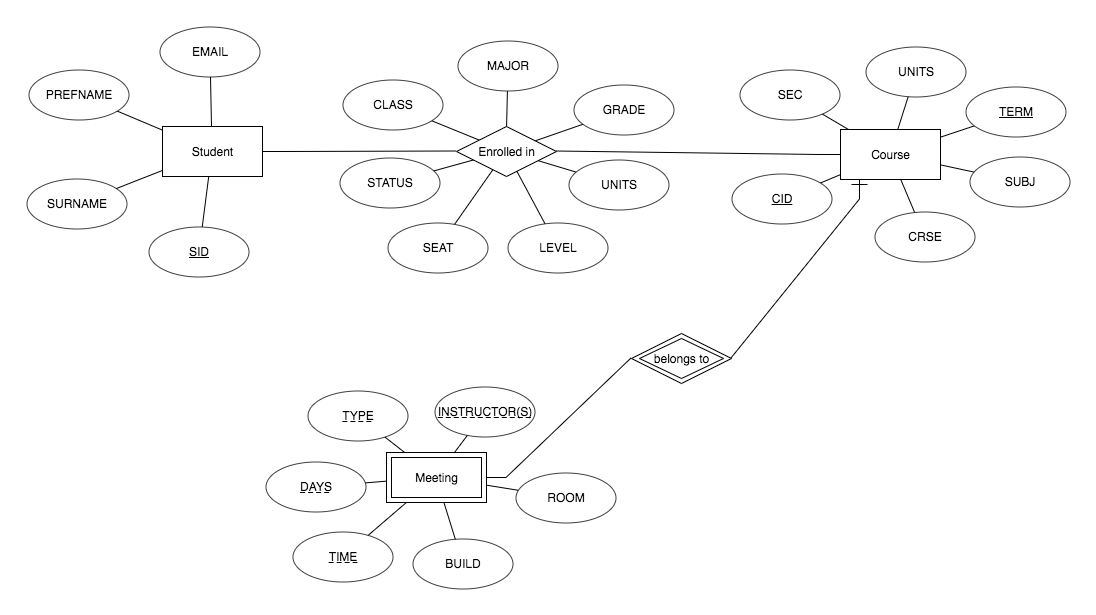
\includegraphics[width=150mm]{erdiagram.png}


 \clearpage
\item Provide a description of the tables in your schema, and their attributes. Make sure you describe how you will store the instructor, student, building, course, etc. information. \\
% Problem 1b goes below

The relations are the following: \\

Course(\underline{CID}, \underline{TERM}, SUBJ, CRSE, SEC, UNITS) \\
Meeting(\underline{CID}, \underline{TERM}, INSTRUCTOR(S), \underline{TYPE}, DAYS, TIME, BUILD, ROOM) \\
Enrolled(\underline{CID}, \underline{TERM}, \underline{SID}, SEAT, LEVEL, UNITS, CLASS, MAJOR, GRADE, STATUS) \\
Student(\underline{SID}, SURNAME, PREFNAME, EMAIL) \\

In the schema we will have four tables: Course, Student, Meeting, and Enrolled. \\

Course: \\
We have the following attributes: CID, TERM, SUBJ, CRSE, SEC, UNITS. CID, TERM, CRSE, and SEC are INT data types. SUBJ and UNITS are VARCHAR data types. The key is $\{CID, TERM\}$. \\

Meeting:\\
We have the following attributes: CID, TERM, INSTRUCTOR(S), TYPE, DAYS, TIME, BUILD, and ROOM. CID and TERM are INT data types. The remaining attributes are stored as VARCHAR. The key is $\{CID, TERM, TYPE\}$. \\

Enrolled: \\
We have the following attributes: CID, TERM, SID, SEAT, LEVEL, UNITS, CLASS, MAJOR, GRADE, and STATUS. CID, TERM, SID, and SEAT are of type INT. UNITS is of type DECIMAL. The rest are of type VARCHAR. The key is $\{CID, TERM, SID\}$. \\

Student: \\
We have the following attributes: SID, SURNAME, PREFNAME, and EMAIL. SID is stored as an INT data type. SURNAME, PREFNAME, and EMAIL are stored as VARCHAR data types. The key is $\{SID\}$. \\ \clearpage
\item What are the functional (and multivalue) dependencies that you expect to hold for each relation if any. If you don't expect any to hold, describe why not. \\
% Problem 1c goes below
The FD's that should hold are the following:  \\

Student: \\
\text{SID} $\,\to\,$ \text{PREFNAME SURNAME EMAIL} \\

Course: \\
\text{CID TERM} $\,\to\,$ \text{SEC UNITS SUBJ CRSE} \\

Enrolled: \\
\text{CID TERM SID} $\,\to\,$ \text{SEAT LEVEL UNITS CLASS MAJOR GRADE STATUS} \\

Meeting: \\
\text{CID TERM TYPE} $\,\to\,$ \text{INSTRUCTOR(S) DAYS TIME BUILD ROOM} \\\\


The MD's that should hold are the following: \\

Student: \\
\text{SID} $\twoheadrightarrow$ \text{PREFNAME SURNAME EMAIL} \\
\text{SID} $\twoheadrightarrow$ \text{PREFNAME} \\
\text{SID} $\twoheadrightarrow$ \text{SURNAME EMAIL} \\
\text{SID} $\twoheadrightarrow$ \text{SURNAME} \\
\text{SID} $\twoheadrightarrow$ \text{PREFNAME EMAIL} \\
\text{SID} $\twoheadrightarrow$ \text{EMAIL} \\
\text{SID} $\twoheadrightarrow$ \text{SURFNAME PREFNAME} \\


Course: \\
\text{CID TERM} $\twoheadrightarrow$ \text{SEC UNITS SUBJ CRSE} \\
\text{CID TERM} $\twoheadrightarrow$ \text{SEC} \\
\text{CID TERM} $\twoheadrightarrow$ \text{UNITS SUBJ CRSE} \\
\text{CID TERM} $\twoheadrightarrow$ \text{UNITS} \\
\text{CID TERM} $\twoheadrightarrow$ \text{SEC SUBJ CRSE} \\
\text{CID TERM} $\twoheadrightarrow$ \text{SUBJ} \\
\text{CID TERM} $\twoheadrightarrow$ \text{SEC UNITS CRSE} \\
\text{CID TERM} $\twoheadrightarrow$ \text{CRSE} \\
\text{CID TERM} $\twoheadrightarrow$ \text{SEC SUBJ UNITS} \\


Enrolled: \\
\text{CID TERM SID} $\twoheadrightarrow$ \text{SEAT LEVEL UNITS CLASS MAJOR GRADE STATUS} \\
\text{CID TERM SID} $\twoheadrightarrow$ \text{SEAT} \\
\text{CID TERM SID} $\twoheadrightarrow$ \text{LEVEL UNITS CLASS MAJOR GRADE STATUS} \\
\text{CID TERM SID} $\twoheadrightarrow$ \text{LEVEL} \\
\text{CID TERM SID} $\twoheadrightarrow$ \text{SEAT UNITS CLASS MAJOR GRADE STATUS} \\
\text{CID TERM SID} $\twoheadrightarrow$ \text{UNITS} \\
\text{CID TERM SID} $\twoheadrightarrow$ \text{SEAT LEVEL CLASS MAJOR GRADE STATUS} \\
\text{CID TERM SID} $\twoheadrightarrow$ \text{CLASS} \\
\text{CID TERM SID} $\twoheadrightarrow$ \text{SEAT LEVEL UNITS MAJOR GRADE STATUS} \\
\text{CID TERM SID} $\twoheadrightarrow$ \text{MAJOR} \\
\text{CID TERM SID} $\twoheadrightarrow$ \text{SEAT LEVEL UNITS CLASS GRADE STATUS} \\
\text{CID TERM SID} $\twoheadrightarrow$ \text{GRADE} \\
\text{CID TERM SID} $\twoheadrightarrow$ \text{SEAT LEVEL UNITS CLASS MAJOR STATUS} \\
\text{CID TERM SID} $\twoheadrightarrow$ \text{STATUS} \\
\text{CID TERM SID} $\twoheadrightarrow$ \text{SEAT LEVEL UNITS CLASS MAJOR GRADE} \\


Meeting: \\
\text{CID TERM TYPE} $\twoheadrightarrow$ \text{INSTRUCTOR(S) DAYS TIME BUILD ROOM} \\
\text{CID TERM TYPE} $\twoheadrightarrow$ \text{INSTRUCTOR(S)} \\
\text{CID TERM TYPE} $\twoheadrightarrow$ \text{DAYS TIME BUILD ROOM} \\
\text{CID TERM TYPE} $\twoheadrightarrow$ \text{DAYS} \\
\text{CID TERM TYPE} $\twoheadrightarrow$ \text{INSTRUCTOR(S) TIME BUILD ROOM} \\
\text{CID TERM TYPE} $\twoheadrightarrow$ \text{TIME} \\
\text{CID TERM TYPE} $\twoheadrightarrow$ \text{INSTRUCTOR(S) DAYS BUILD ROOM} \\
\text{CID TERM TYPE} $\twoheadrightarrow$ \text{BUILD} \\
\text{CID TERM TYPE} $\twoheadrightarrow$ \text{INSTRUCTOR(S) DAYS TIME ROOM}
\text{CID TERM TYPE} $\twoheadrightarrow$ \text{ROOM} \\
\text{CID TERM TYPE} $\twoheadrightarrow$ \text{INSTRUCTOR(S) DAYS TIME BUILD} \\
 \clearpage
\end{enumerate}

\section*{Part 2} 
Write a program to load the grade data into a PostgreSQL database called FakeUData that follows your schema.
You {\bf MUST} use the database called FakeUData, and should assume it will already be created for you without any tables or data in it.
You may {\bf NOT} hardcode usernames in your code, use the USER environmental variable instead if user is needed.
Your program can be written in C++ or python, you may {\bf NOT} use standalone SQL or text files that hold your queries. 
You may {\bf NOT} use shell calls to implement your program.
All your queries need to be in your code. 
If you choose to make a C++ program, you must include a makefile and call the program loadfakeu. 
Include a readme file with descriptions of any issues/problems. 
If you choose to make a python program you must specify which version of python you used, and must provide a loadfakeu bash script to launch your python program.
The loadfakeu program {\bf MUST} be able to take one optional argument (the directory where the CSV data files will be located). 
If the argument is omitted, the default is the current working directory.
Scripts that require greater than 10 minutes to load all of the data may lose points. 
\clearpage

\section*{Part 3}
Write another program to query your database to calculate the following values, put the results in your write up, some may be best described with a chart instead of raw values. 
Name your program queryfakeu, it must output the data values for the following queries. 
The query program does not have to do everything in the SQL queries, but should limit the amount of data transfered. 
For example it is acceptable to have one SQL query for each unit number (1 - 20) for 3a, but it would be unacceptable to pull all student data on a per student basis and calculate the results. 
\begin{enumerate}[label=\alph*.]
\item Calculate the percent of students that attempt 1 - 20 units of ABC or DEF per quarter for every unit increment (e.g. 1, 2, 3, ...). \\
% Problem 2a goes below

\begin{verbatim}
units, percent
(1, 12.181803682578057)
(2, 2.6949890244567842)
(3, 7.75633034916078)
(4, 64.56725300830615)
(5, 6.164351939292445)
(6, 0.3408084547358524)
(7, 0.36892934940001765)
(8, 0.5275815610873973)
(9, 0.17628023520819955)
(10, 0.3382901656614496)
(11, 1.406464448053992)
(12, 1.4060447332082584)
(13, 0.0)
(14, 0.0)
(15, 0.0)
(16, 0.0)
(17, 0.0)
(18, 0.0)
(19, 0.0)
(20, 0.0)

\end{verbatim} \clearpage
\item Find the easiest and hardest instructors based upon the grades of all the students they have taught in their courses. Provide their name and the average grade they assigned. (Ignore P/NP, S/NS grades) \\
% Problem 2b goes below

\begin{verbatim}
    
('EASIEST PROFESSOR:', 'Donaldson, Matthew C.', 'AVG GRADE =', 'A')
('HARDEST PROFESSOR:', 'White, Jose E.', 'AVG GRADE =', 'F')
\end{verbatim} \clearpage
\item Calculate the average GPA for the students that take each number of units from part a. Assume that the grades have standard grade points (A+ = 4.0, A = 4.0, A- = 3.7, B+ = 3.3...). \\
% Problem 2c goes below
 \clearpage
\item Find the courses with the highest and lowest pass rates. Assume that F, NP, and NS are not passing grades. \\
% Problem 2d goes below

\begin{verbatim}
Courses with the highest pass rate:
subj, course, pass_rate
('ABC', 110, 1.0)
('ABC', 111, 1.0)
('ABC', 114, 1.0)
('ABC', 215, 1.0)
('ABC', 223, 1.0)
('ABC', 225, 1.0)
('ABC', 231, 1.0)
('ABC', 233, 1.0)
('ABC', 244, 1.0)
('ABC', 249, 1.0)
('ABC', 250, 1.0)
('ABC', 252, 1.0)
('ABC', 255, 1.0)
('ABC', 259, 1.0)
('ABC', 260, 1.0)
('ABC', 302, 1.0)
('ABC', 303, 1.0)
('ABC', 311, 1.0)
('ABC', 313, 1.0)
('ABC', 315, 1.0)
('ABC', 317, 1.0)
('ABC', 318, 1.0)
('ABC', 321, 1.0)
('ABC', 323, 1.0)
('ABC', 326, 1.0)
('ABC', 327, 1.0)
('ABC', 328, 1.0)
('ABC', 333, 1.0)
('ABC', 334, 1.0)
('ABC', 340, 1.0)
('ABC', 341, 1.0)
('ABC', 342, 1.0)
('ABC', 343, 1.0)
('ABC', 345, 1.0)
('ABC', 346, 1.0)
('ABC', 349, 1.0)
('ABC', 351, 1.0)
('ABC', 352, 1.0)
('ABC', 353, 1.0)
('ABC', 357, 1.0)
('ABC', 358, 1.0)
('ABC', 359, 1.0)
('ABC', 361, 1.0)
('ABC', 362, 1.0)
('ABC', 364, 1.0)
('ABC', 368, 1.0)
('ABC', 369, 1.0)
('ABC', 372, 1.0)
('ABC', 373, 1.0)
('ABC', 374, 1.0)
('ABC', 377, 1.0)
('DEF', 105, 1.0)
('DEF', 213, 1.0)
('DEF', 216, 1.0)
('DEF', 217, 1.0)
('DEF', 218, 1.0)
('DEF', 224, 1.0)
('DEF', 236, 1.0)
('DEF', 237, 1.0)
('DEF', 240, 1.0)
('DEF', 255, 1.0)
('DEF', 260, 1.0)
('DEF', 272, 1.0)
('DEF', 278, 1.0)
('DEF', 282, 1.0)
('DEF', 287, 1.0)
('DEF', 288, 1.0)
('DEF', 293, 1.0)
('DEF', 295, 1.0)
('DEF', 298, 1.0)
('DEF', 302, 1.0)
('DEF', 303, 1.0)
('DEF', 304, 1.0)
('DEF', 305, 1.0)
('DEF', 306, 1.0)
('DEF', 307, 1.0)
('DEF', 310, 1.0)
('DEF', 313, 1.0)
('DEF', 314, 1.0)
('DEF', 316, 1.0)
('DEF', 319, 1.0)
('DEF', 320, 1.0)
('DEF', 322, 1.0)
('DEF', 323, 1.0)
('DEF', 324, 1.0)
('DEF', 325, 1.0)
('DEF', 328, 1.0)
('DEF', 329, 1.0)
('DEF', 332, 1.0)
('DEF', 333, 1.0)
('DEF', 337, 1.0)
('DEF', 338, 1.0)
('DEF', 339, 1.0)
('DEF', 341, 1.0)
('DEF', 343, 1.0)
('DEF', 345, 1.0)
('DEF', 348, 1.0)
('DEF', 349, 1.0)
('DEF', 351, 1.0)
('DEF', 352, 1.0)
('DEF', 353, 1.0)
('DEF', 354, 1.0)
('DEF', 355, 1.0)
('DEF', 362, 1.0)
('DEF', 363, 1.0)
('DEF', 364, 1.0)
('DEF', 365, 1.0)
('DEF', 366, 1.0)
('DEF', 368, 1.0)
('DEF', 369, 1.0)
('DEF', 375, 1.0)
('DEF', 376, 1.0)
('DEF', 378, 1.0)
('DEF', 380, 1.0)
('DEF', 381, 1.0)
('DEF', 382, 1.0)
('DEF', 386, 1.0)
('DEF', 387, 1.0)
('DEF', 388, 1.0)
('DEF', 390, 1.0)
('DEF', 393, 1.0)
('DEF', 397, 1.0)
('DEF', 398, 1.0)
('DEF', 401, 1.0)
('DEF', 403, 1.0)
('DEF', 404, 1.0)
('DEF', 408, 1.0)
('DEF', 410, 1.0)
('DEF', 411, 1.0)
('DEF', 412, 1.0)
('DEF', 414, 1.0)
('DEF', 419, 1.0)
('DEF', 420, 1.0)
('DEF', 422, 1.0)
('DEF', 423, 1.0)
('DEF', 424, 1.0)
('DEF', 425, 1.0)

Courses with the lowest pass rate:
subj, course, pass_rate
('DEF', 290, 0.2)
\end{verbatim} \clearpage
\item Find the list of courses that must be cross listed as they have the same meeting times during the normal quarters. Only list the pair once, put the course name/number string in alphabetically order of the pairs. \\
% Problem 2e goes below
 \clearpage
\item Find the major that performs the best/worst on average in ABC courses. Repeat the analysis for DEF courses as well. \\
% Problem 2f goes below
 \clearpage
\item Find the top 5 majors that students transfer from into ABC. What is the percent of students from each of those majors compared to overall transfers? \\
% Problem 2g goes below

\begin{center}
    \begin{tabular}{|c| c|}
        \hline 
        Major & Percent \\
        \hline
        DEF2 & 18.0890126754959 \\
        \hline
        OT16 & 12.4117546751549 \\
        \hline
        DEF1 & 12.2992099130336 \\
        \hline
        OT35 & 5.6977206843631\\
        \hline
        OT26 & 4.85192974478486 \\
        \hline
    \end{tabular}
\end{center}
 \clearpage
\item Find the top 5 majors that students transfer to from ABC. What is the percent of students to each of those majors compared to overall transfers out? \\
% Problem 2h goes below
 \clearpage
\end{enumerate}

\section*{Part 4}
Extra credit: The Efficient XML Interchange (EXI) is a format for the compact representation of XML information. 
The CSV files provided for this assignment have been consolidated into a single EXI file (HW4Grades.exi) that is available in the resources section of Canvas. 
Implement a separate program that it can load the database from the EXI file. 
You may {\bf NOT} use shell calls, or creation of external temporary files for this part.
Name your program or bash script loadfakeuexi.
\clearpage

\section*{Part 5}
Extra credit: Additional queries/query program.
\begin{enumerate}[label=\alph*.]
\item Find the courses that appear to be prerequisites for ABC 203, ABC 210, and ABC 222. For this problem list the courses that the X\% of students have taken for every 5\% increment from 50\% - 100\% prior to taking the course. (Add this output to your query program.)\\
% Problem 2a goes below
 \clearpage
\item Write a program that will find an open room for course expansion. The program must prompt for term, CID, and number students to add. The room(s) returned should be ordered from best to worst fit with up to 5 results. Assume that each room capacity is the maximum number of students listed for any particular meeting in the data files (don't forget that lectures may be split across multiple CIDs). Name this program findroomfakeu.
% Problem 2b goes below
 \clearpage
\end{enumerate}



\end{document}